\documentclass[11pt]{article}

\topmargin -.5in
\textheight 9in
\oddsidemargin -.25in
\evensidemargin -.25in
\textwidth 7in
\usepackage{amsmath}
\usepackage{listings}
\usepackage{fancyvrb}
\usepackage{indentfirst}
\usepackage{hyperref}
\usepackage{graphicx}
\usepackage{multicol}
\graphicspath{ {./} }
\usepackage{multicol}
\usepackage{subcaption}
\graphicspath{ {img/} }
\newcommand{\numpy}{{\tt numpy}}
\usepackage[utf8x]{inputenc}

\begin{document}
\title{Tugas Kelompok Analisis Numerik : Optimisasi}
\author{Kelompok B09}
\date{April 2019}
\maketitle

% \begin{multicols}{1}
\section{Introduction}
\label{sec:Intro}
Tugas kelompok Analisis Numerik yang ke-3 ini memiliki topik umum optimisasi. Hal - hal yang perlu kami lakukan pada tugas berikut ini dapat dibagi menjadi 3 bagian, yaitu : 
\begin{enumerate}
    \item Implementasi
    \item Eksperimen Teoritis
    \item Eksperimen Aplikatif
\end{enumerate}

Ketiga bagian tersebut berkaitan dengan proses optimisasi terhadap suatu rumus matematika yang sering digunakan pada suatu riset (seperti \textit{Ackley Function} dan \textit{Lennard-Jones Potential Function}), yang mana proses optimisasi tersebut adalah proses pencarian solusi paling optimal (umumnya yang paling minimal atau paling maksimal). Pada tugas ini, kami akan menggunakan beberapa fungsi optimisasi tak berkendala yang diimplementasikan menggunakan MATLAB/Octave dan memasukkan rumus yang mau dicari nilai optimalnya ke dalam fungsi optimisasi.

\section{Why?}
Selain karena ingin lulus mata kuliah analisis numerik, kami juga tertarik dengan bagaimana hasil dari pengaplikasian metode optimisasi terhadap rumus - rumus yang sering digunakan dalam berbagai penelitian dan penghitungan, seperti \textit{Ackley Function} dan \textit{Lennard-Jones Potential Function}. Apakah kami berhasil membuat algoritma optimisasi dengan tepat sehingga hasilnya optimal? Atau apakah algoritmanya masih salah sehingga hasilnya masih belum optimal (misal terjebak di \textit{local minima}) ? Kami berharap kami bisa menemukan jawaban pertanyaan - pertanyaan tersebut dengan menyelesaikan tugas kelompok ini.

\section{Content}
\subsection{Aktivitas 1: Implementasi}

\medskip

Aktivitas pertama adalah membuat atau mengimplementasikan tiga buah fungsi yang masing-masing merepresentasikan metode untuk menyelesaikan masalah optimisasi. Fungsi tersebut adalah:

\begin{enumerate}
    \item Optimisasi Newton : Menerima input berupa $TOL$, angka tebakan awal $x_{0}$, fungsi $f(x)$, fungsi turunan pertama $∇f(x)$, dan fungsi turunan kedua $H_{f}(x)$,
    \item \textit{Steepest Descent} : Menerima input berupa $TOL$, tebakan awal $x_{0}$, fungsi $f(x)$ dan fungsi turunan pertama $∇f(x)$, dan
    \item \textit{Quasi-Newton SR-1} : Menerima input berupa $TOL$, tebakan awal $x_{0}$, fungsi $f(x)$ dan fungsi turunan pertama $∇f(x)$
\end{enumerate}

\medskip

Pada ketiga fungsi diatas, TOL merepresentasikan batas nilai terkecil akurasi perbedaan yang dapat diterima sebagai solusi optimal (batas toleransi). Selain itu, dalam implementasi metode \textit{Quasi-Newton SR-1} dan \textit{Steepest Descent}, dibutuhkan rumus yang dapat menentukan besar langkah yang diambil pada setiap iterasi ($a$) yaitu \textit{Armijo Backtracking Line Search}. Untuk kode implementasi ketiga fungsi tersebut, dapat dilihat pada lampiran kode.

\subsection{Aktivitas 2 : Eksperimen Teoritis}

\medskip

Aktivitas kedua adalah eksperimen teoritis untuk mengecek implementasi fungsi yang dibuat di aktivitas pertama. \textit{Ackley Function} merupakan fungsi $non-convex$ yang digunakan untuk melakukan pengujian terhadap performa algoritma optimisasi sehingga kami mencoba memeriksa akurasi algoritma optimisasi kami dengan rumus ini. Berikut merupakan rumus fungsi Ackley :

\medskip

\[
f(x) =  - 20exp(-0.2\sqrt{\frac{1}{d} \sum_{i=1}^{d} x_{i}^{2}} ) - exp(\frac{1}{d}\sum_{i=1}^{d}cos(2x_{i}\pi)) + 20 + exp(1))
\]

\medskip

Rumus tersebut membutuhkan suatu parameter $d$ sebagai dimensi. Soal menspesifikasikan $d ∈ \{2, 8, 32\}$ dan domain pengujian algoritma ditentukan di interval $x_{i} ∈ [-30, 30]$, dimana dipilih 20 angka sebagai nilai $x_{i}$ dari selang tersebut menggunakan rumus $(b-a)/n$ dengan $b = 30$, $a = 30$ dan $n = 20$. Pada kasus ini, diperbolehkan kemunculan berulang di antara nilai $x_{i}$ namun duplikasi nilai diminimalkan.

\medskip

Aktivitas 2 memiliki tujuan untuk melakukan pengetesan terhadap ketiga algoritma optimisasi yang telah dibuat sebelumnya, untuk setiap nilai $d$ masing-masing. Proses ini dapat juga disebut \textit{benchmarking}, yaitu menilai performa dari algoritma yang telah dibuat. \textit{Benchmarking} ini dilakukan dengan mencatat waktu dari masing-masing metode pada aktivitas 1 terhadap perhitungan dalam menentukan nilai minimum global fungsi Ackley. Untuk penulisan rumus Ackley tiap dimensinya, dapat dilihat pada lampiran kode.

\medskip
%van, udah bisa di submit belom?
Untuk $d = 2$, kami menggunakan nilai tebakan awal berupa vektor [1;5]. Untuk ketiga metode tersebut, kami menggunakan TOL $10^{5}$

Dalam menentukan ketiga nilai fungsi tersebut, kami mengalami beberapa kesulitan. Selain karena sumber daya mesin yang terbatas, nilai alpha yang semakin mengecil menyebabkan langkah yang diambil pada setiap iterasi menjadi sangat kecil. Akibatnya, kami tidak dapat menentukan waktu dan konvergensi dari metode \textit{steepest-descent}.
\begin{itemize}
    \item \textit{Quasi-Newton SR1} : f(x) konvergen ke 9.8265, time = 0.067182
    \item \textit{Newton method} : f(x) konvergen ke 10.258, time = 0.0081348
    \item \textit{Steepest Descent} : f(x) konvergen ke -, time = -
\end{itemize}

\medskip
Untuk $d = 8$, kami menggunakan nilai tebakan awal berupa vektor [ 2;3;5;7;11;13;17;19]. Untuk ketiga metode tersebut, kami menggunakan TOL $10^{5}$

Dalam menentukan ketiga nilai fungsi tersebut, kami mengalami beberapa kesulitan. Selain karena sumber daya mesin yang terbatas, nilai alpha yang semakin mengecil menyebabkan langkah yang diambil pada setiap iterasi menjadi sangat kecil. Akibatnya, kami tidak dapat menentukan waktu dan konvergensi dari metode \textit{steepest-descent}.

\begin{itemize}
    \item untuk quasi newton sr1 f(x) konvergen ke 17.925, time = 0.13909
    \item untuk newton method f(x) konvergen ke  17.925, time = 0.018294
    \item untuk steepest descent f(x) konvergen ke -, time = -
\end{itemize}

\medskip
Untuk $d = 32$, kami menggunakan nilai tebakan awal berupa vektor
[1;2;3;4;5;6;7;8;9;10;11;12;13;14;15;16;17;18;19;20;1;2;3;4;5;6;7;8;9;10;11;12]
dengan TOL sebesar $10^{5}$, sehingga kami memperoleh hasil yang cukup cepat untuk ketiga metode.
\begin{itemize}
    \item untuk quasi newton sr1 f(x) konvergen ke 17.54683000209215, time 6.785392761230469e-02
    \item untuk newton method f(x) konvergen ke  17.54682999685339, time 8.850407600402832e-02
    \item untuk steepest descent f(x) konvergen ke 17.54683000061292, time 3.243279457092285e-02
\end{itemize}

Waktu dihitung dengan menggunakan \textit{tic toc} Octave dan menggunakan satuan detik.

\medskip

\subsection{Aktivitas 3 : Eksperimen Aplikatif}

\medskip
Aktivitas 3 adalah eksperimen aplikatif yang melakukan optimisasi terhadap \textit{Lennard-Jones Potensial Function} (selanjutnya akan disebut \textit{Lennard-Jones Function}) yang berbunyi :

\[
    U(r) = 4\varepsilon\bigg(\Big(\frac{\sigma}{r}\Big)^{12} - \Big(\frac{\sigma}{r}\Big)^6\bigg)
\]

\subsubsection{Aktivitas 3.1}
Berdasarkan fungsi tersebut, akan ditentukan nilai minimum $r$ yang akan menyebabkan $U(r)$ minimum. Cara mencari $r_{min}$ dengan mencari solusi dari $U'(r) = 0$.

\[
    U'(r) = \frac{24\varepsilon\sigma^6(r^6-2\sigma^6)}{r^{13}} = 0
\]
\[
    r = \sigma\sqrt[6]{2}
\]

Didapatkan $r_{min} = \sigma\sqrt[6]{2}$, energi minimum dapat diperoleh sebagai $E_{min} = U(r_{min})$.

\[
    E_{min} = 4\varepsilon\bigg(\Big(\frac{\sigma}{\sigma\sqrt[6]{2}}\Big)^{12} - \Big(\frac{\sigma}{\sigma\sqrt[6]{2}}\Big)^6\bigg) = -\varepsilon
\]

\medskip

Selanjutnya akan ditunjukkan bahwa :

\[
U(r) = -E_{min}\bigg(\Big(\frac{r_{min}}{r}\Big)^{12} - 2\Big(\frac{r_{min}}{r}\Big)^6 \bigg)
\]

\[
4\varepsilon\bigg(\Big(\frac{\sigma}{r}\Big)^{12} - \Big(\frac{\sigma}{r}\Big)^6\bigg) = -(-\varepsilon)\bigg(\Big(\frac{\sigma\sqrt[6]{2}}{r}\Big)^{12} - 2\Big(\frac{\sigma\sqrt[6]{2}}{r}\Big)^6 \bigg)
\]

\[
4\varepsilon\bigg(\Big(\frac{\sigma}{r}\Big)^{12} - \Big(\frac{\sigma}{r}\Big)^6\bigg) = \varepsilon\bigg(\Big4(\frac{\sigma}{r}\Big)^{12} - 4\Big(\frac{\sigma}{r}\Big)^6 \bigg)
\]

\[
4\varepsilon\bigg(\Big(\frac{\sigma}{r}\Big)^{12} - \Big(\frac{\sigma}{r}\Big)^6\bigg) = 4\varepsilon\bigg(\Big(\frac{\sigma}{r}\Big)^{12} - \Big(\frac{\sigma}{r}\Big)^6 \bigg)
\]

Terbukti bahwa $U(r)$ dapat ditulis ulang sebagai $-E_{min}\bigg(\Big(\frac{r_{min}}{r}\Big)^{12} - 2\Big(\frac{r_{min}}{r}\Big)^6 \bigg)$.

\subsubsection{Aktivitas 3.2}

Aktivitas ini akan menentukan optimisasi numerik dan visualisasinya dengan menggunakan metode Newton untuk mencari posisi ekulibrium dari $n=6$ buah atom.

\medskip

Fungsi yang hendak dioptimisasi ini sendiri bernama \textit{Lennard-Jones Potential Function}, yaitu fungsi yang menghitung energi potensial antar atom berdasarkan jarak. Fungsi ini kemudian akan dioptimisasi dengan mencari nilai jarak ($r$) yang minimal. Dan karena jarak itu sendiri ditentukan dari posisi tiap atomnya, maka bagian ini juga meminta kami untuk mencari posisi ekuilibrium untuk $n=6$ buah atom. Fungsi pendukung terdapat di halaman kode.

\medskip

Menurut penelitian oleh \textit{Alfred Werner} mengenai kestabilan atom-atom yang membentuk oktahedral, energi minimum dari keenam atom tersebut akan mengikuti pola seperti berikut : Jika atom pertama berada di posisi $(0, 0, 0)$, maka posisi atom - atom selanjutnya adalah $(0, 0, 2K), (0, K, K), (0, -K, K), (K, 0, K)$, dan $(-K, 0, K)$. Oleh karena itu, $k$ akan berfungsi sebagai variabel bebas dari \textit{Lennard-Jones Function} yang akan dioptimisasi dengan metode Newton. Dengan kata lain, \textit{Lennard-Jones Function} dapat ditulis ulang sebagai berikut :

\[
3 * \bigg(\frac{1}{(4*k^2)^6} - \frac{2}{(4*k^2)^3}\bigg) + 12 * \bigg(\frac{1}{(2*k^2)^6} - \frac{2}{(2*k^2)^3}\bigg)
\]
\newline
\newline
\textbf{Bagian A}

\medskip

Dengan mengambil tebakan awal $k = 0.5$, dan $TOL$ sebesar $10^{-13}$. Kami memilih nilai $TOL$ yang cukup relaks utamanya disebabkan ketidakmampuan komputer kami menghitung nilai iterasi yang cukup kecil, sehingga kami menghentikan proses iterasinya saat mencapai nilai yang menurut kami tidak signifikan lagi. Dari proses iterasi didapatkan nilai $k = 0.7039468473095744$ dan nilai \textit{Lennard-Jones Function $(f(x))$} sebesar $-12.71206225680934$, yang hampir mendekati nilai -13 yang merupakan nilai optimum.

\medskip

Gradien dari fungsi $(∇f(x))$  memiliki nilai $-0.4260415283315921*10^{-14}$ (hampir mendekati nol), sementara hessian $H_{f}$ dari fungsi $(H_{f}(x))$ memiliki nilai 1847.007976901734 (nilai hessian positif menunjukkan positif definit, yang berarti nilainya minimum). Berikut adalah hasil \textit{plotting} dari iterasi yang algoritma kami lakukan :

% ini gue bingung cara multicols gambar
\begin{multicols}{2}
%nah bisa
    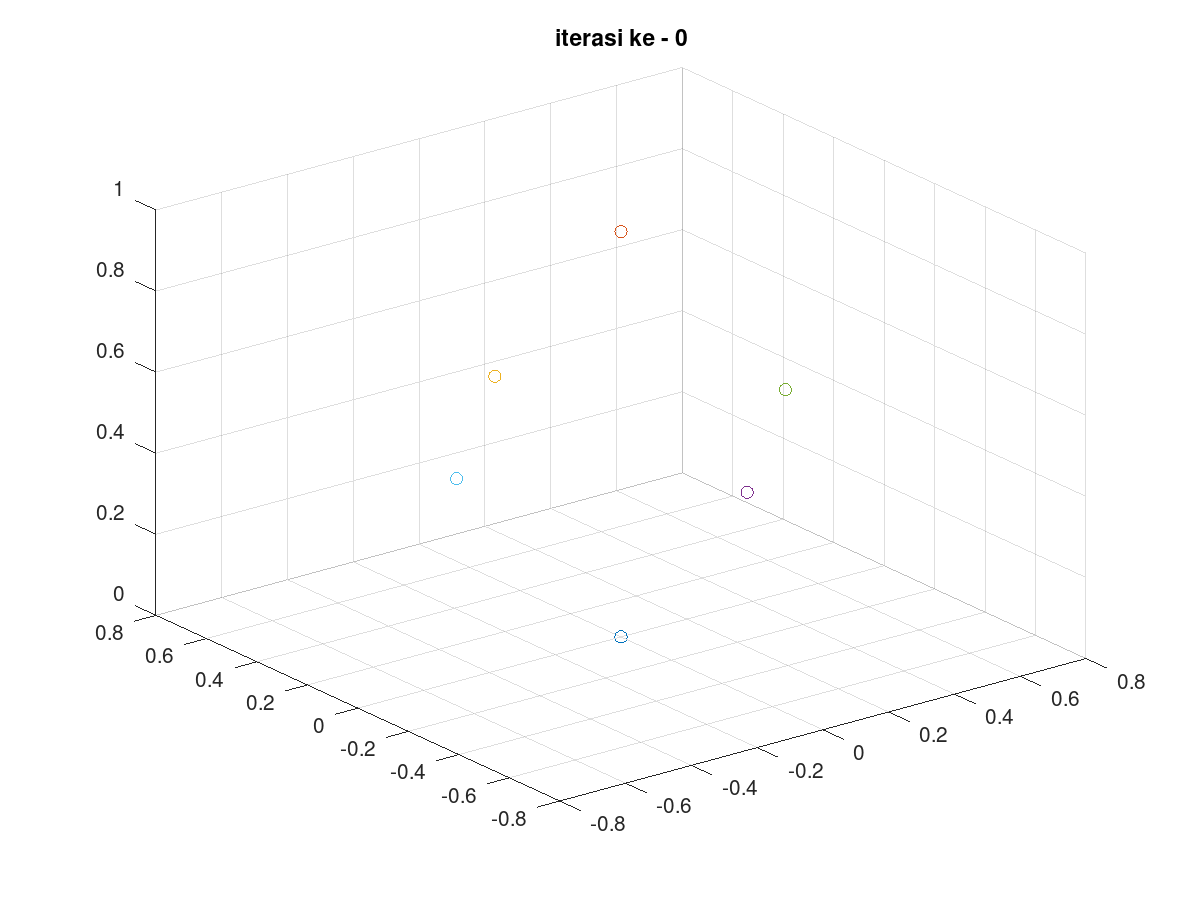
\includegraphics[width=8cm]{img/Iterasi00.png}
    
    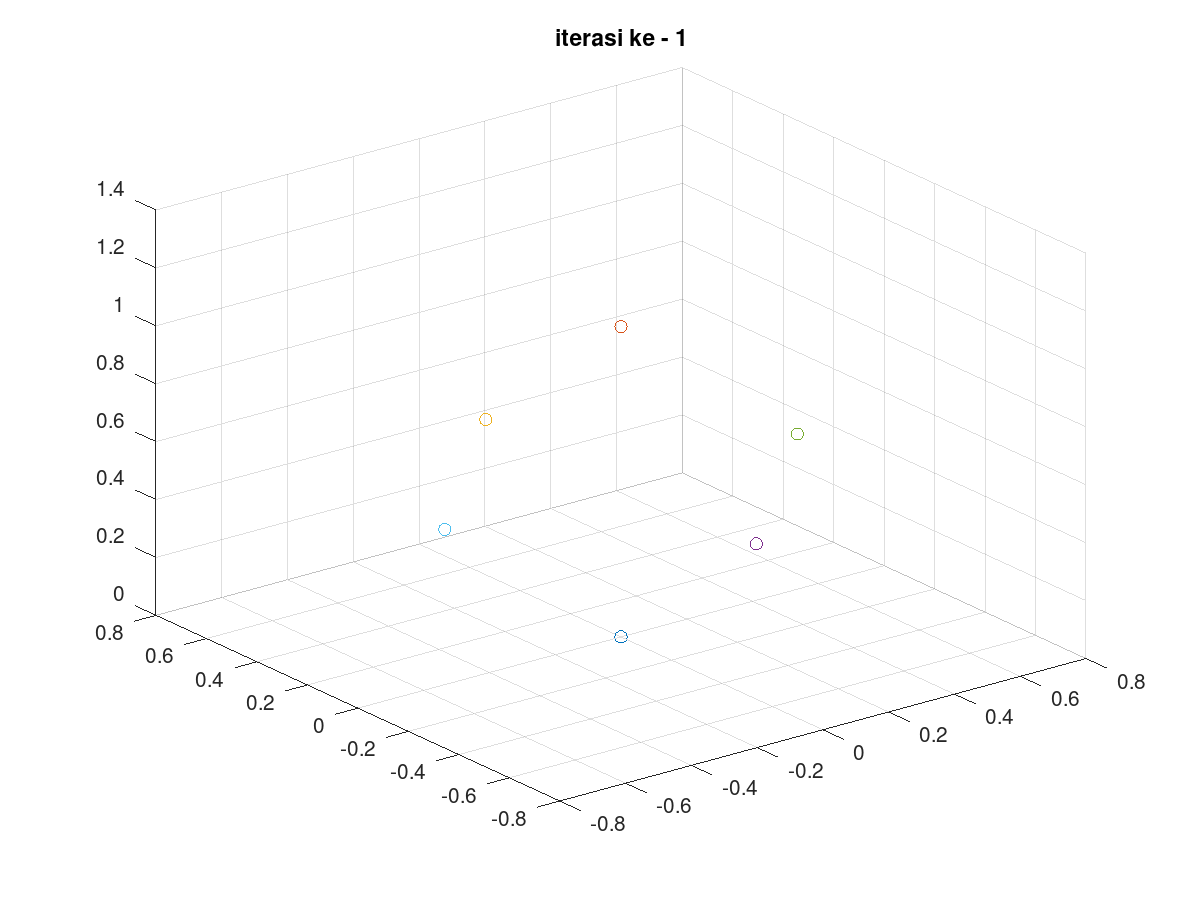
\includegraphics[width=8cm]{img/Iterasi01.png}

    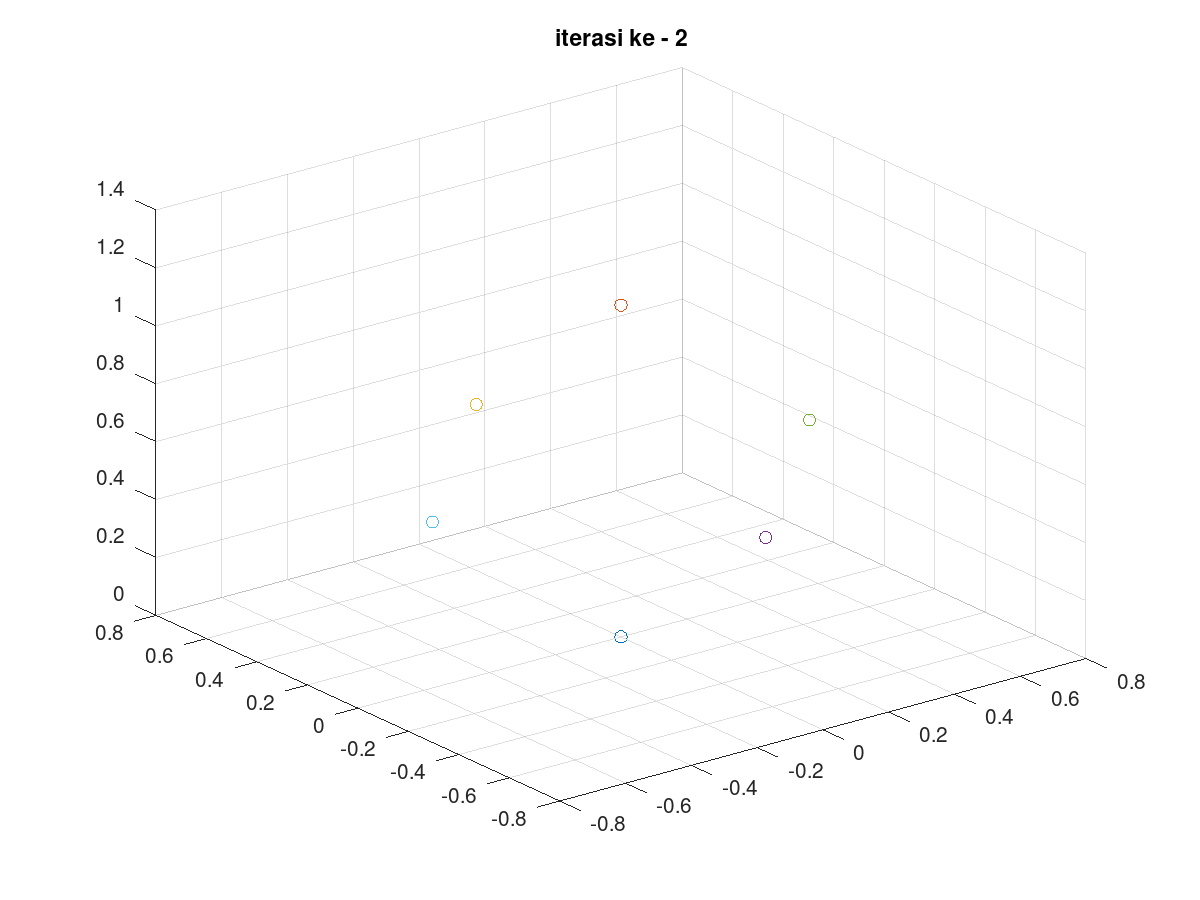
\includegraphics[width=8cm]{img/Iterasi02.png}
% kayaknya caption hapus aja deh
% di gambar udah ada tulisan iterasi ke berapa
%ok

    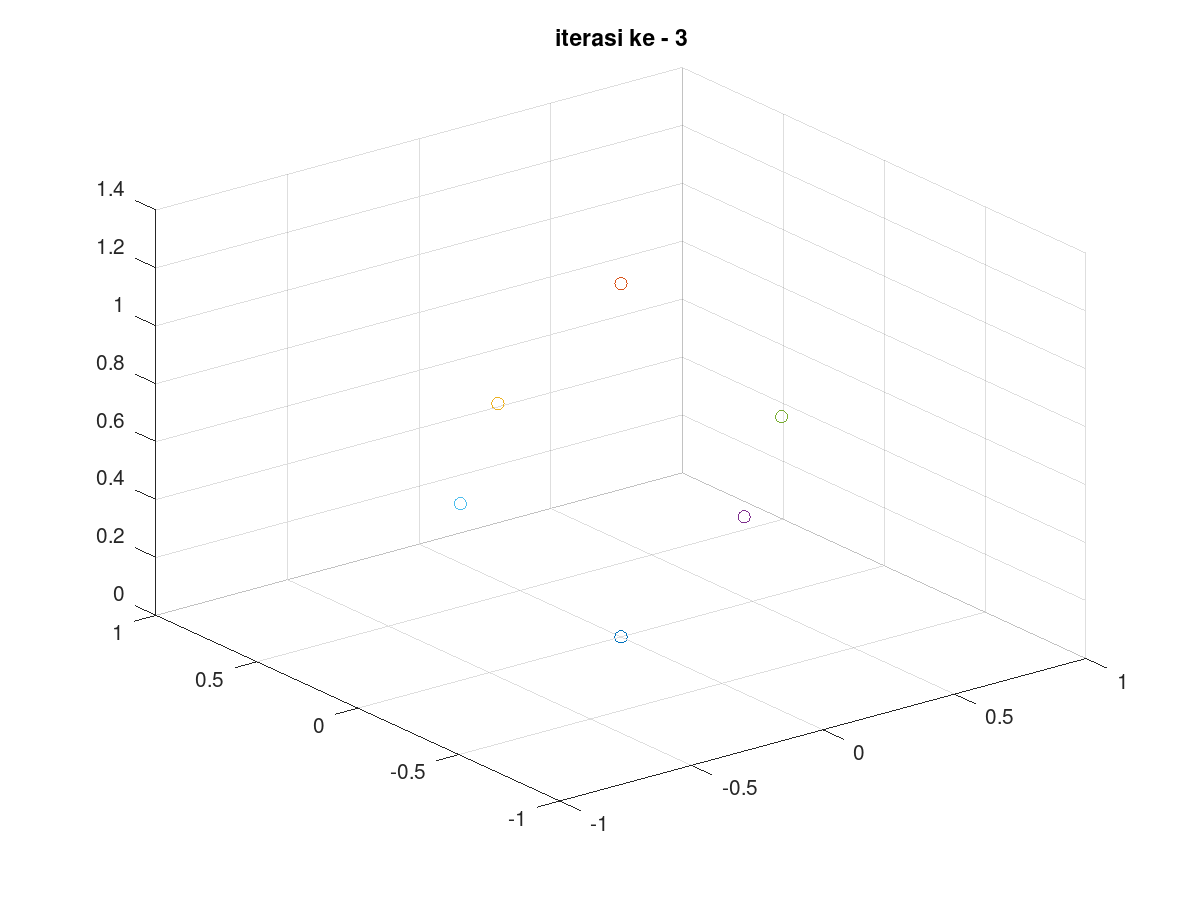
\includegraphics[width=8cm]{img/Iterasi03.png}

    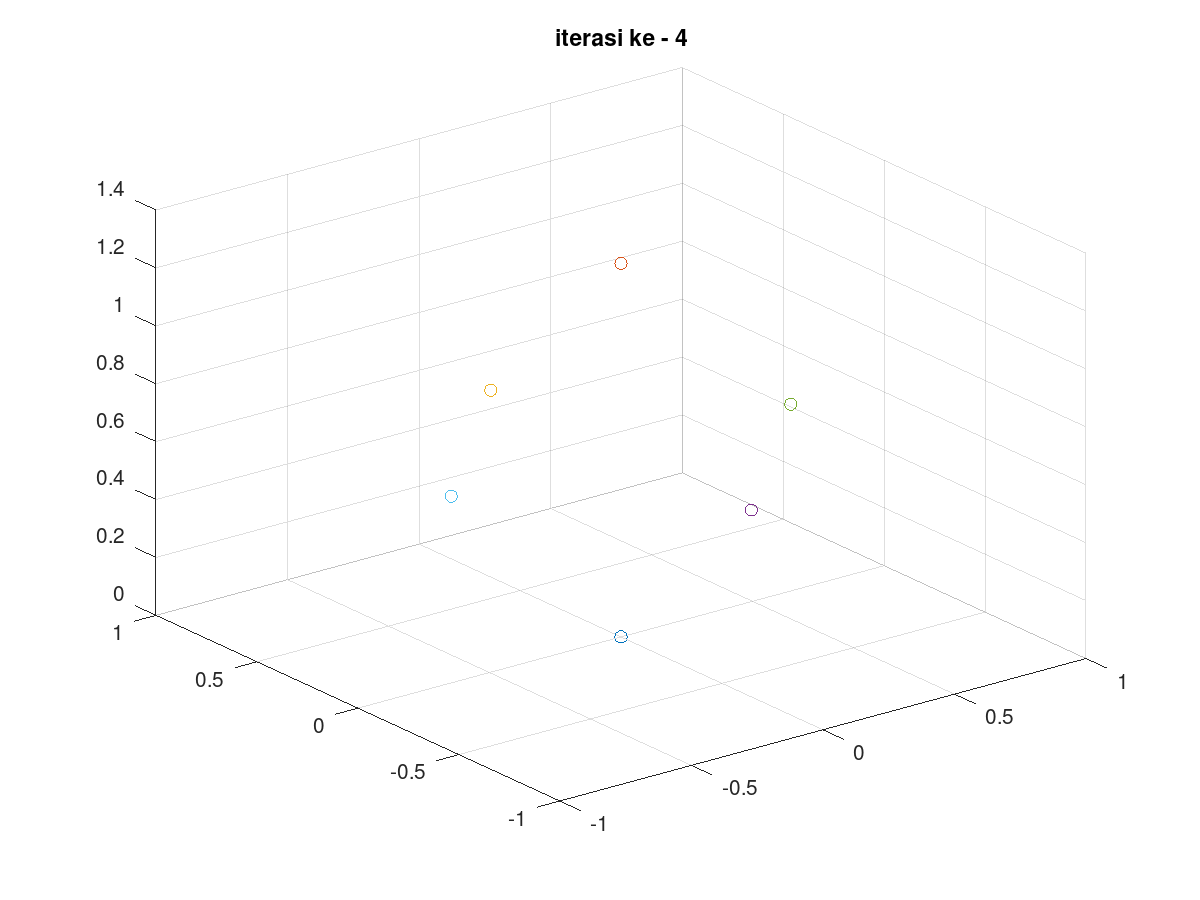
\includegraphics[width=8cm]{img/Iterasi04.png}

    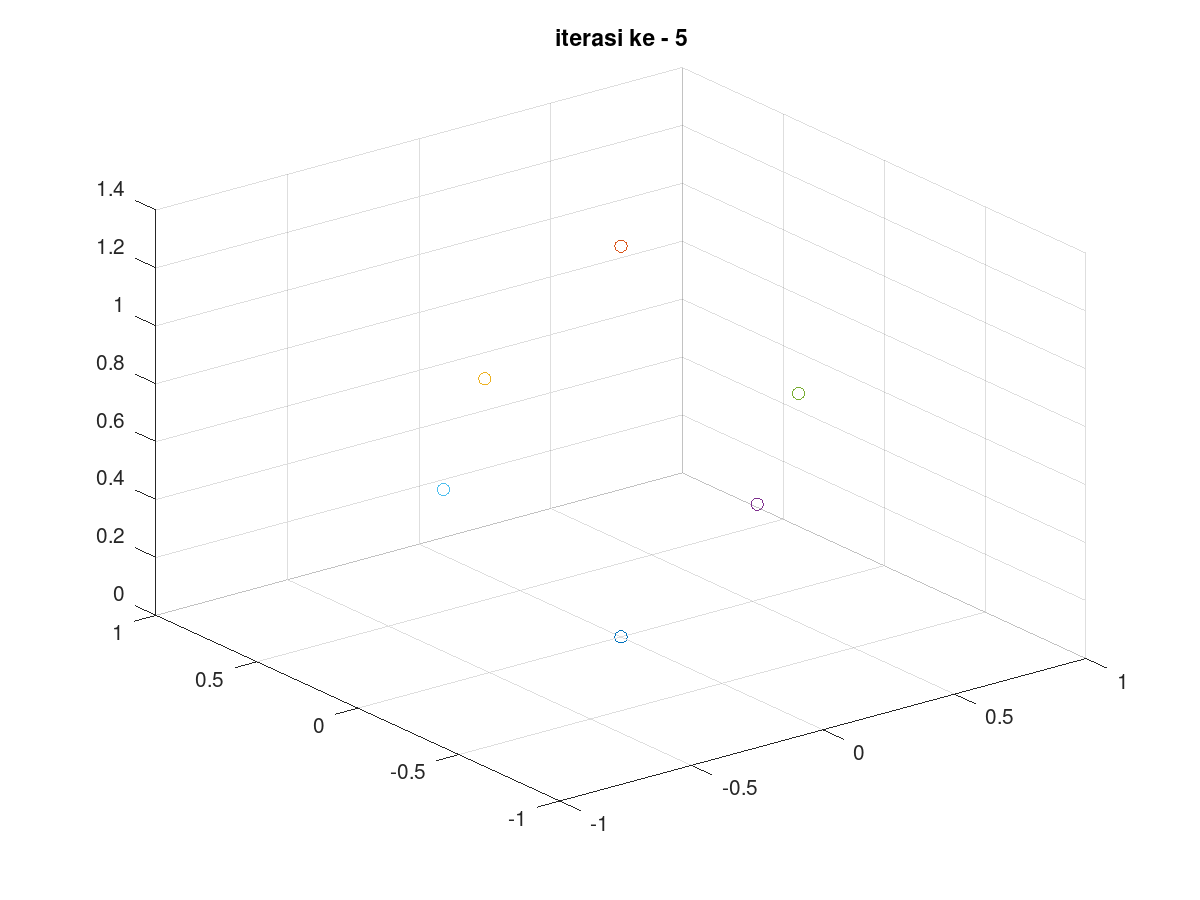
\includegraphics[width=8cm]{img/Iterasi05.png}

    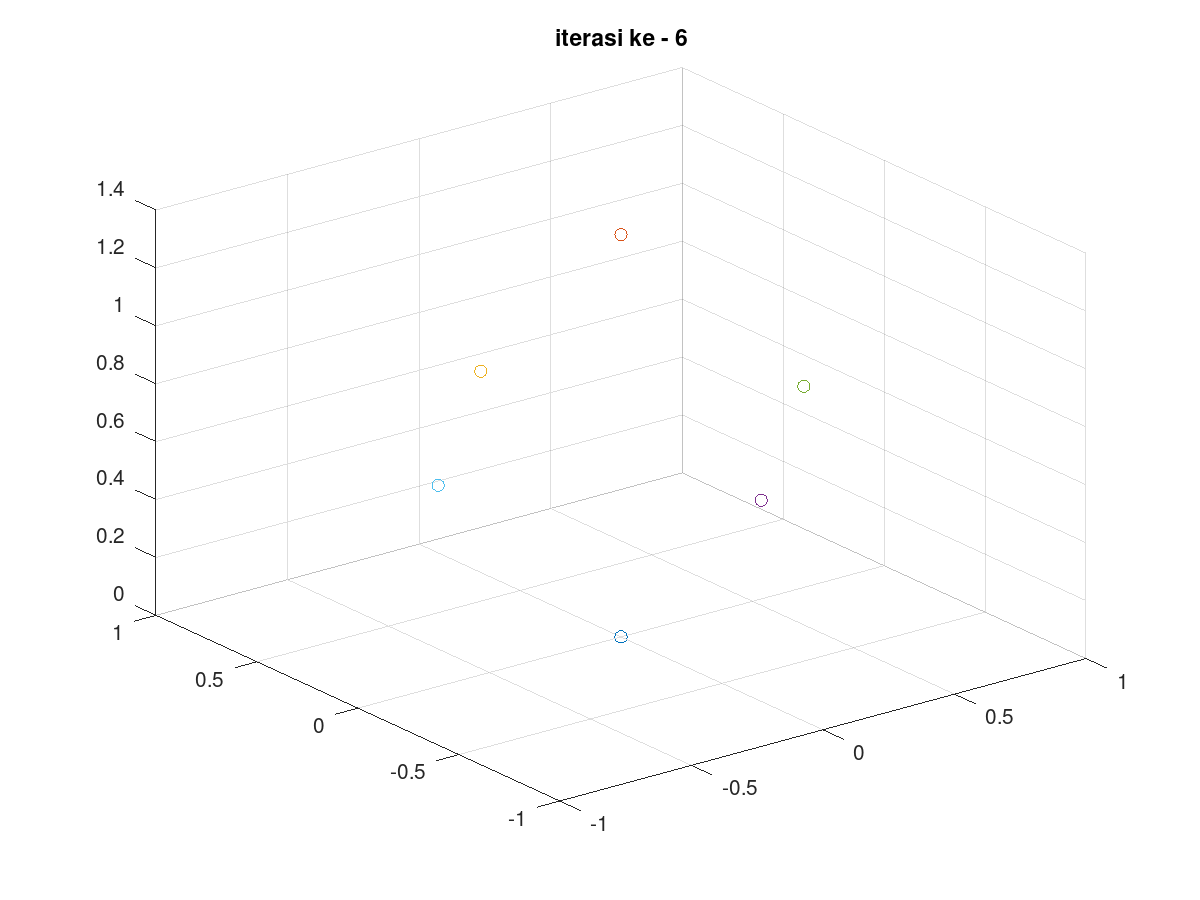
\includegraphics[width=8cm]{img/Iterasi06.png}

    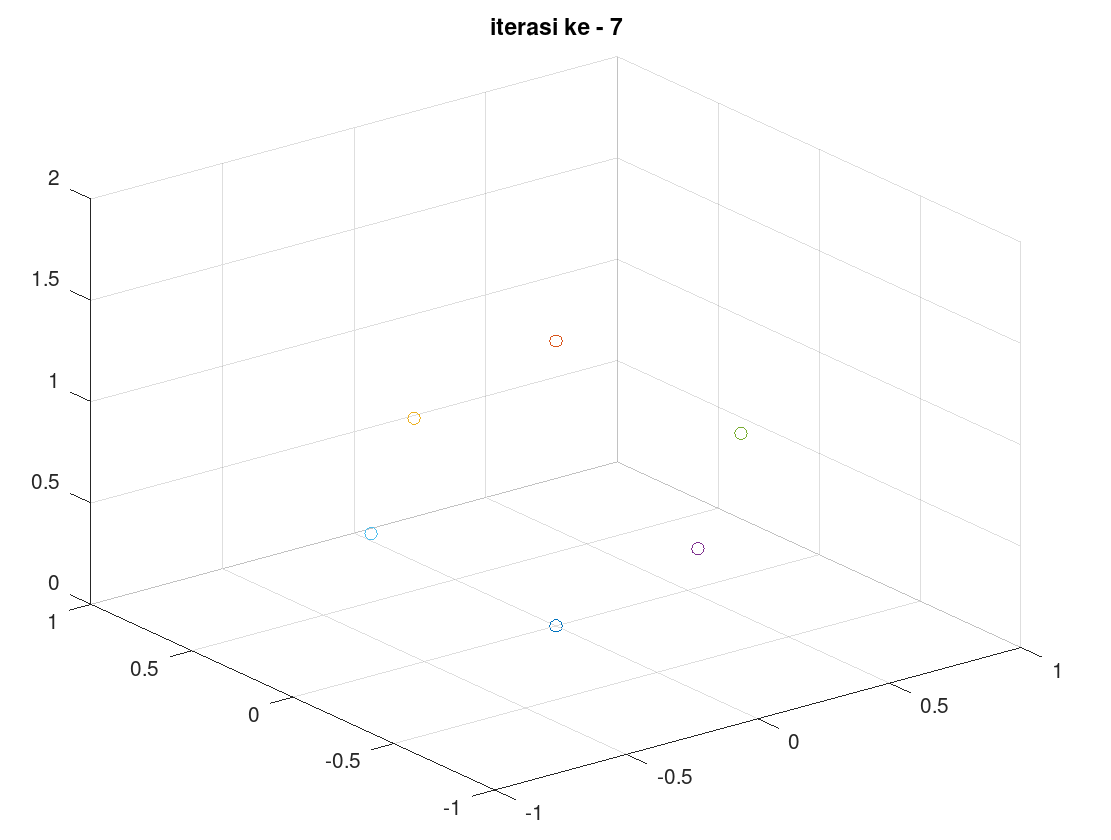
\includegraphics[width=8cm]{img/Iterasi07.PNG}

    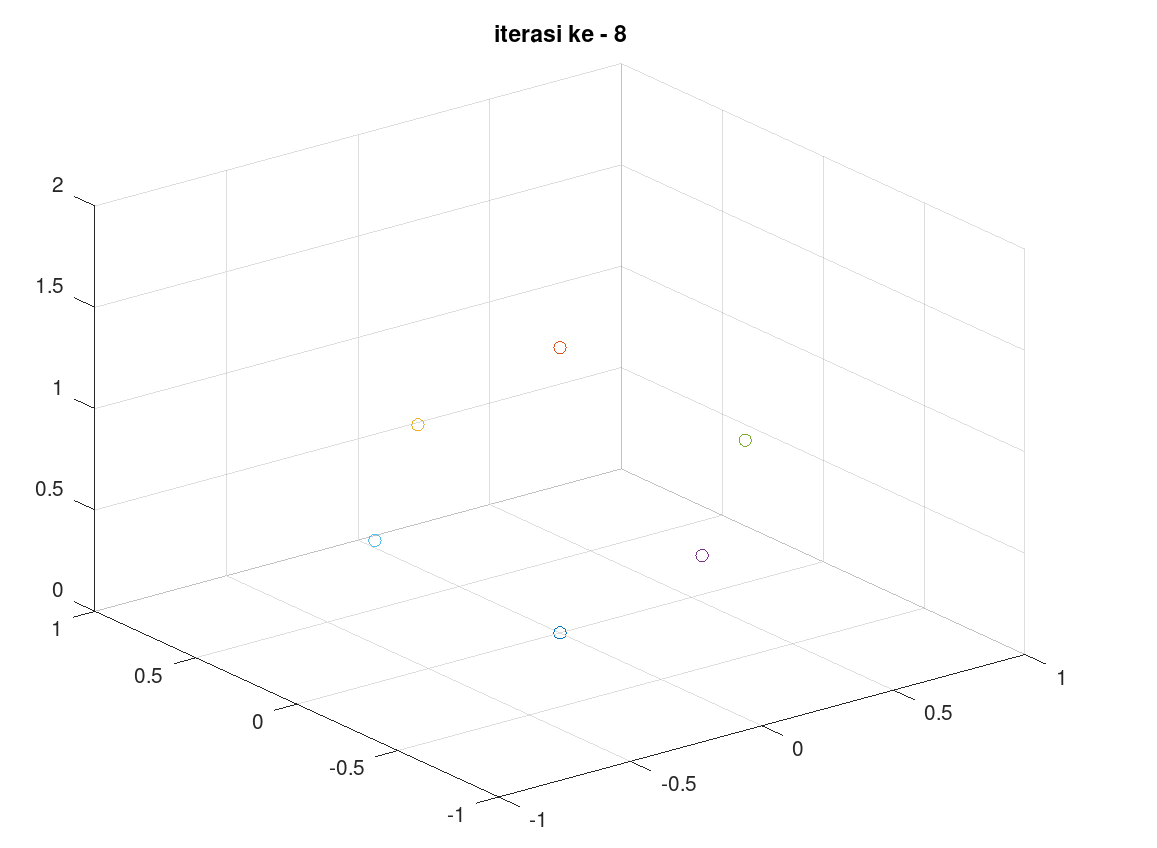
\includegraphics[width=8cm]{img/Iterasi08.PNG}

    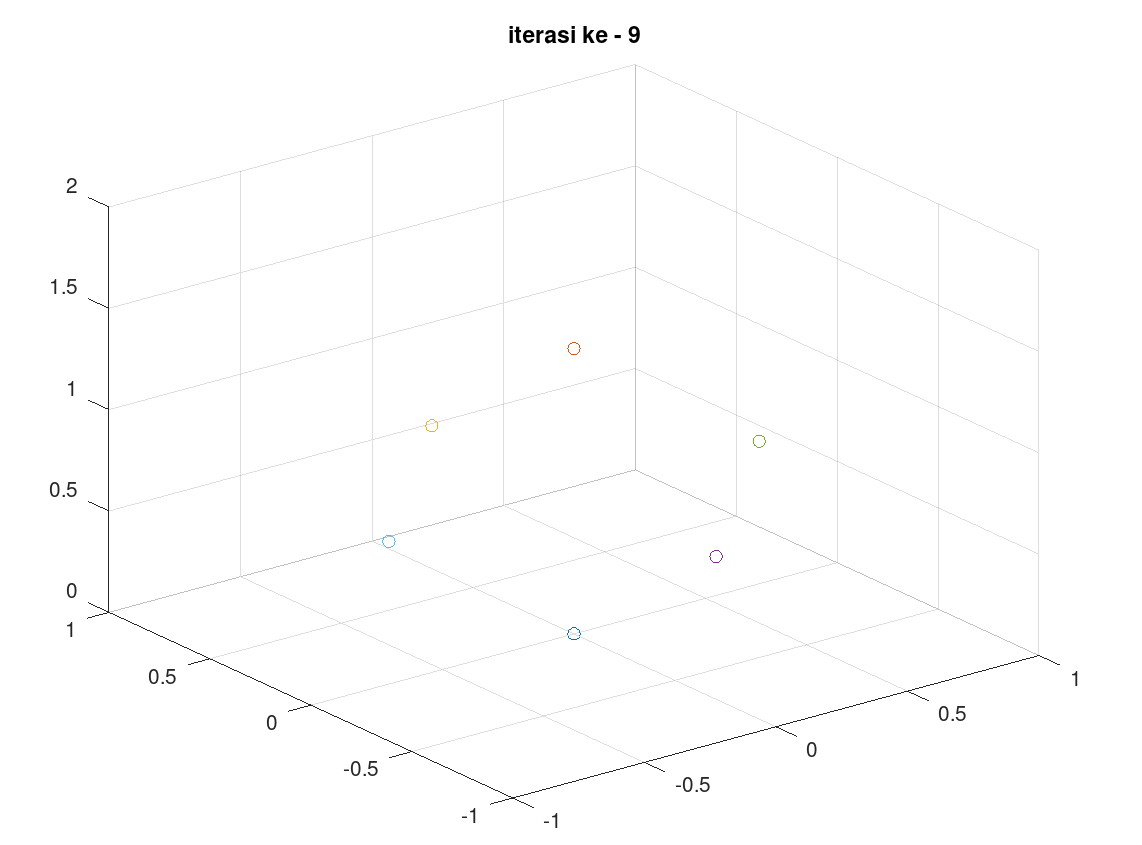
\includegraphics[width=8cm]{img/Iterasi09.PNG}

    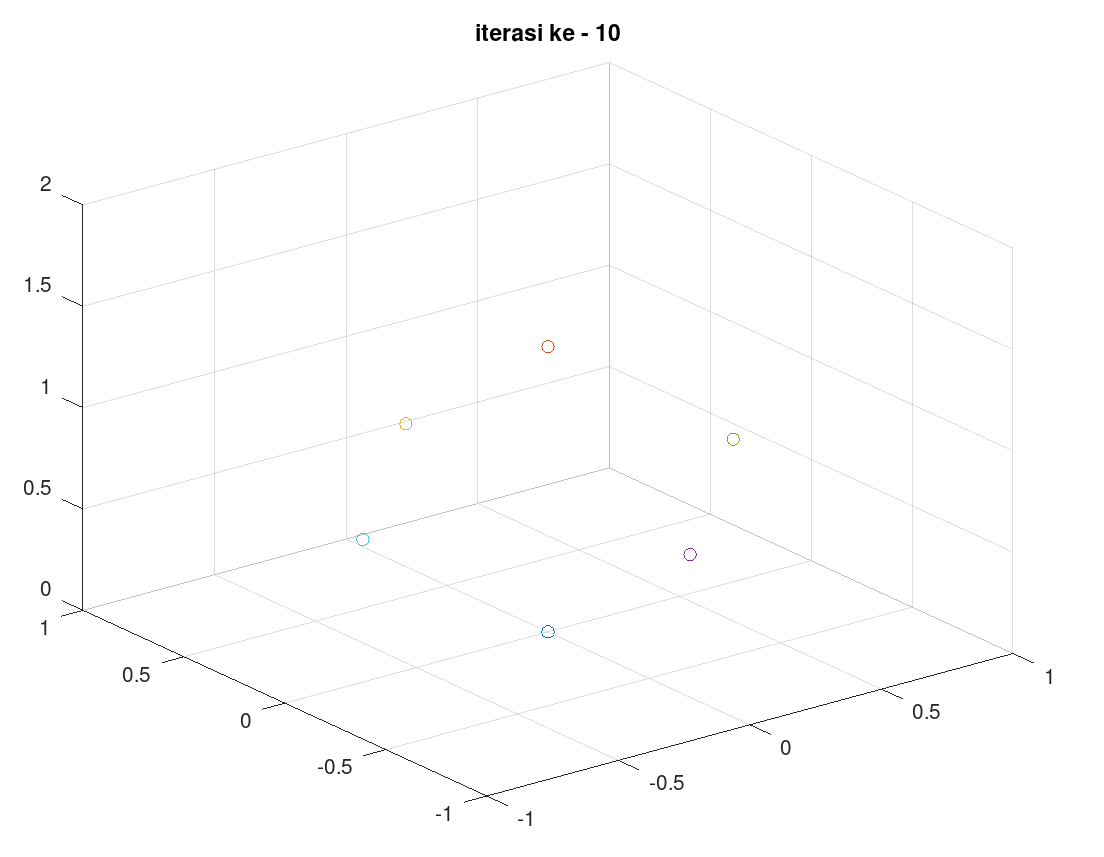
\includegraphics[width=8cm]{img/Iterasi10.PNG}

    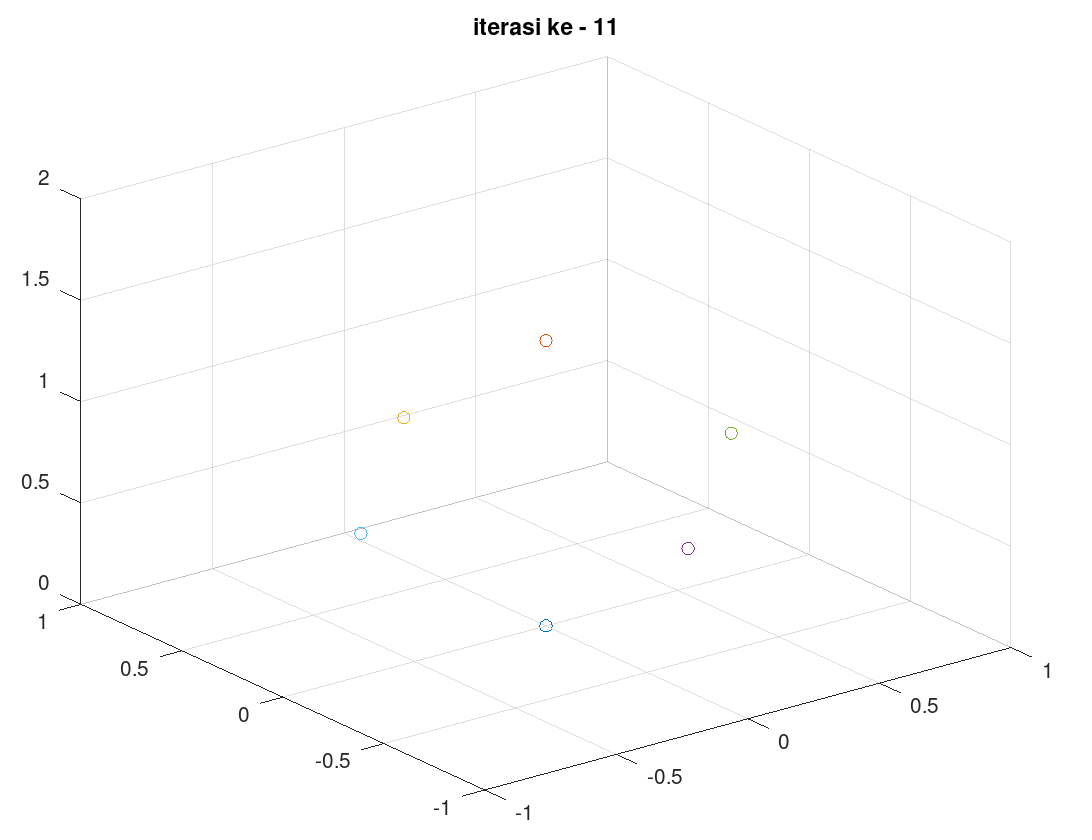
\includegraphics[width=8cm]{img/Iterasi11.PNG}
\end{multicols}

\textbf{Bagian B}

\medskip

Dengan mengacu kepada model oktahedral yang dicetuskan oleh Alfred Werner, didapatkan nilai $k = 0.7039468473095744$ sebagai nilai minimum global. Kami juga sudah mencoba 100 poin acak titik tebakan awal dan masing-masing titik tebakan tersebut akan konvergen ke titik $k = 0.7039468473095744$ atau ke sebuah k lain yang memiliki nilai \textit{Lennar-Jones Function} yang lebih besar. Untuk memperjelas, dapat dilihat grafik nilai \textit{Lennar-Jones Function} yang dimana digunakan titik antara $[0.6, 10]$ karena fungsi mendekati nilai $infinity$ saat fungsi mendekati nol sehingga hanya akan menunjukkan grafik tegak lurus.

\centerline{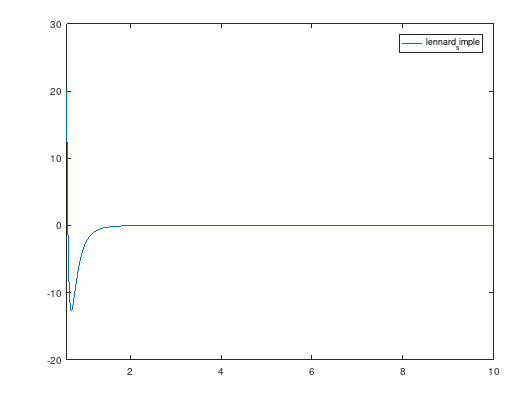
\includegraphics[width=10cm]{img/LJ_Graph_rapi.png}}

\textbf{Bagian C} 

\medskip

Dengan mengambil $k = 10$ dan $TOL = 10^{-13}$, fungsi akan terjebak di minimum lokal ($k =\\110.6254514129296$ dengan nilai fungsi lennard jones sebesar $-1.687931745003293e-12$).


\section{Conclusion}
Dari pengerjaan tugas ini, kami menjadi lebih paham mengenai proses dan tujuan dari optimisasi numerik. Dengan adanya optimisasi numerik, dapat dicari nilai terbaik berdasarkan preferensi yang akan memaksimalkan potensi dari suatu fungsi. Kami juga mengetahui bahwa komputasi yang dilakukan untuk optimisasi membutuhkan waktu yang tidak sedikit (terutama jika \textit{resource} mesin terbatas). Oleh karena itu, diperlukan algoritma yang cukup efektif dan optimal agar optimisasi dapat tercapai.

\section{Reference}
\begin{enumerate}
    \item Damanik, Raja (2019). \textit{Slide Optimisasi}. Retrieved from Numerical Analysis Course year 2018/2019 (Link : https://scele.cs.ui.ac.id/course/view.php?id=625)
    \item Doye, Jonathan (1997). \textit{Table of global minima LJ$_{n}$ for N < 150} 
    \item Sauer, Timothy (2012). \textit{Numerical Analysis}. Boston, MA: Pearson Education
    \item https://onlinelibrary.wiley.com/doi/abs/10.1002/anie.199103231
    \item https://www.wolframalpha.com (Untuk beberapa penurunan fungsi)

\end{enumerate}

% \end{multicols}{1}
\end{document}
